\documentclass[10pt, a4paper,spanish]{article}
\usepackage[utf8]{inputenc}

\usepackage{varwidth}
\usepackage{graphicx}

\usepackage[T1]{fontenc} % Use 8-bit encoding that has 256 glyphs
\usepackage{microtype} % Slightly tweak font spacing for aesthetics

\usepackage[hmarginratio=1:1,top=32mm,columnsep=20pt]{geometry} % Document margins
\usepackage[hang, small,labelfont=bf,up,textfont=it,up]{caption} % Custom captions under/above floats in tables or figures
\usepackage{booktabs} % Horizontal rules in tables
\usepackage{float} % Required for tables and figures in the multi-column environment - they need to be placed in specific locations with the [H] (e.g. \begin{table}[H])
\usepackage{hyperref} % For hyperlinks in the PDF

\usepackage{lettrine} % The lettrine is the first enlarged letter at the beginning of the text
\usepackage{paralist} % Used for the compactitem environment which makes bullet points with less space between them

\usepackage{fancyhdr} % Headers and footers
\pagestyle{fancy} % All pages have headers and footers
\fancyhead{} % Blank out the default header
\fancyfoot{} % Blank out the default footer
\fancyhead[C]{ Mayo 2016 $\bullet$ JumpVa $\bullet$ Informe Final} % Custom header text
\fancyfoot[RO,LE]{\thepage} % Custom footer text

%----------------------------------------------------------------------------------------
%	TITLE SECTION
%----------------------------------------------------------------------------------------

\title{\vspace{-15mm}\fontsize{24pt}{10pt}\selectfont\textbf{Informe Final}} % Article title

\author{
\large
\textsc{Sergio García Prado}\\[2mm] % Your name
\normalsize Universidad de Valladolid \\ % Your institution
\vspace{-5mm}
}
\date{\today}

%----------------------------------------------------------------------------------------

\begin{document}
	\begin{titlepage}
	\centering
		%\includegraphics[width=0.15\textwidth]{example-image-1x1}\par\vspace{1cm}
		{\scshape\LARGE Universidad de Valladolid \par}
		\vspace{1cm}
		{\scshape\Large Prácticas en Empresa\par}
		\vspace{1.5cm}
		{\huge\bfseries Brooktec\par}
		\vspace{2cm}
		{\large
		\textsc{Sergio García Prado\textsubscript}\\[2mm] % Your name
		\vspace{-5mm}
		}

		\vfill

	% Bottom of the page
		{\large \today\par}
	\end{titlepage}

	\thispagestyle{fancy} % All pages have headers and footers

%----------------------------------------------------------------------------------------
%	TABLE OF CONTENTS
%----------------------------------------------------------------------------------------

	\tableofcontents
	\newpage

%----------------------------------------------------------------------------------------
%	TEXT
%----------------------------------------------------------------------------------------



    \section{Datos Generales de la Práctica}



    \section{Breve Descripción de la Empresa}



    \section{Memoria de Actividades}



    \section{Conclusiones}



    \newpage
    \section{Declaración de Responsabilidad}

        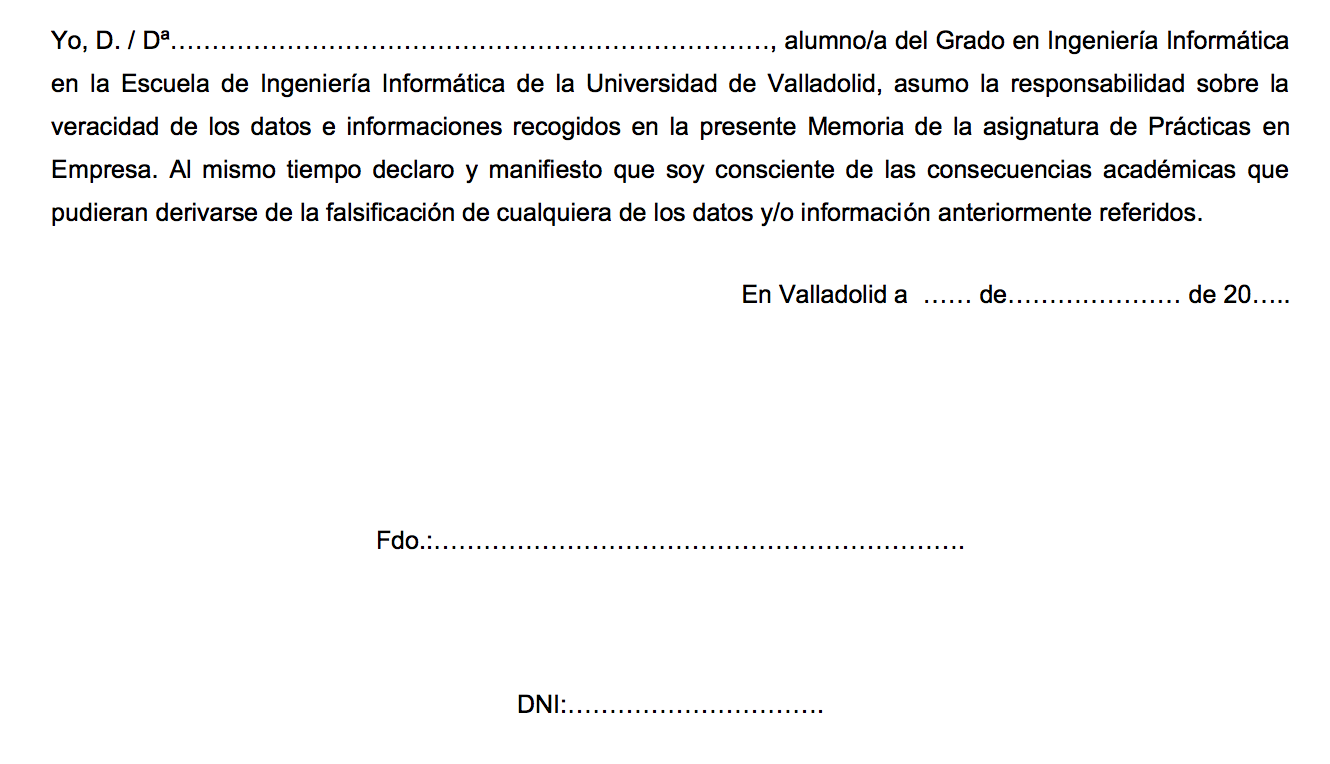
\includegraphics[width=\textwidth]{res/responsibility-declaration}



\end{document}
